\documentclass[titlepage,12pt]{article}

\usepackage[utf8]{inputenc}
\usepackage[brazil]{babel}
\usepackage[T1]{fontenc}
\usepackage{url}
\usepackage{verbatim}
\usepackage{xspace}
\usepackage{graphicx}
\usepackage{wrapfig}

\newcommand{\CEU}{\textsc{C\'{e}u}\xspace}

\title{ Uma Plataforma de Baixo Consumo de Energia, Flexível e Barata para a
        Internet das Coisas }

\author{PROPONENTE:                                     \\
Francisco Figueiredo Goytacaz Sant'Anna                 \\
francisco@ime.uerj.br                                   \\
\\\\
INSTITUIÇÃO DE EXECUÇÃO:                                \\
Departamento de Informática e Ciências da Computação    \\
Instituto de Matemática e Estatística (IME)             \\
Universidade Estadual do Rio de Janeiro (UERJ)          \\
\\\\
Chamada Universal MCTIC/CNPq 2018 
}

\begin{document} 

\maketitle

%\begin{abstract} \end{abstract}

%%%%%%%%%%%%%%%%%%%%%%%%%%%%%%%%%%%%%%%%%%%%%%%%%%%%%%%%%%%%%%%%%%%%%%%%%%%%%%%
% a) Identificação do projeto, incluindo título, palavras-chave e resumo;
%%%%%%%%%%%%%%%%%%%%%%%%%%%%%%%%%%%%%%%%%%%%%%%%%%%%%%%%%%%%%%%%%%%%%%%%%%%%%%%

\section{Identificação do Projeto}

\subsection{Título}

Uma Plataforma de Baixo Consumo de Energia, Flexível e Barata para a Internet
das Coisas

%A Low-Power, Flexible, and Cheap Platform for the Internet of Things

\subsection{Palavras-Chave}

internet das coisas, eficiência energética, linguagem síncrona

%iot, arduino, low power, synchronous language

\subsection{Resumo}

De acordo com a Agência Internacional de Energia (AIE)~\cite{iea.data}, o
número de dispositivos conectados deve atingir 50 bilhões até 2020 com a
expansão da Internet das Coisas (IoT).
A maior parte do consumo de energia nesses dispositivos será em
\emph{modo de espera} (aka \emph{standby mode}), quando eles não estão
transmitindo ou processando dados.
Em particular, o modo de espera é responsável por aproximadamente 10--15\% do
consumo residencial.
Também estima-se que as emissões de $CO_2$ relacionadas ao modo de espera
mundiais seja equivalente às de 1 milhão de carros.

Os efeitos alarmantes do consumo em modo de espera, aliados ao crescimento
estimado da IoT, tornou o modo de espera para dispositivos conectados um dos
seis pilares do \emph{Plano de Ação para Eficiência Energética do G20}%
\footnote{G20's Energy Efficiency Action Plan: \url{https://www.iea-4e.org/projects/g20}}.
No entanto, o uso efetivo do modo de espera requer grandes esforços de software
e hardware para detectar períodos de inatividade nos dispositivos, identificar
periféricos que devem permanecer ligados, e aplicar os modos mais econômicos
sempre que possível.

Este projeto tem como principal objetivo desenvolver uma plataforma de hardware
e software de baixo consumo de energia para pesquisa e educação em Internet das
Coisas.

No que diz respeito ao software, iremos adotar a linguagem de programação
reativa \CEU~\cite{ceu.sensys13}, a qual estamos desenvolvendo durante os
últimos 8 anos, e que tem como alvo sistemas embarcados restritos.
%
\CEU é baseada no modelo de concorrência síncrono, que troca poder por
confiabilidade e possui um modelo de tempo mais simples que cobre a maioria dos
requisitos de aplicações IoT.
%
Nesse modelo, todas as reações ao mundo externo são computadas em tempo finito,
garantindo que as aplicações sempre chegam a um estado ocioso que é suscetível
ao modo de espera.
%
A linguagem já possui suporte recente básico a tratamento de interrupções e
gerenciamento de energia automático.
Em testes preliminares, já alcançamos economias entre 20 e 90\% para aplicações
escritas puramente em \CEU.

No que diz respeito ao hardware, os requisitos principais são o baixo custo e
flexibilidade da plataforma.
%
As soluções completas de hardware atuais são acessíveis mas pouco flexíveis,
pois tipicamente possuem componentes SMD montados na placa.
Em particular, os módulos de rádio são previamente determinados, criando uma
barreira para a pesquisa.
Mesmo que muitas dessas soluções sejam abertas, o custo dos componentes é alto
para compras em pequenas quantidades e o método de montagem não é adequado para
experimentação.
%
A nossa proposta visa projetar uma solução flexível e de baixo custo baseada em
microcontroladores e módulos "de platereira" no mercado brasileiro.

%%%%%%%%%%%%%%%%%%%%%%%%%%%%%%%%%%%%%%%%%%%%%%%%%%%%%%%%%%%%%%%%%%%%%%%%%%%%%%%
% b) Dados do proponente e equipe;
% d) Instituição(ões) participante(s);
%%%%%%%%%%%%%%%%%%%%%%%%%%%%%%%%%%%%%%%%%%%%%%%%%%%%%%%%%%%%%%%%%%%%%%%%%%%%%%%

\section{Equipe e Instituições}

\begin{itemize}
    \item Francisco Figueiredo Goytacaz Sant'Anna
    \begin{itemize}
        \item \textbf{Função:} \\
              Pesquisador Proponente e Coordenador
        \item \textbf{E-mail:} \\
              \url{francisco@ime.uerj.br}
        \item \textbf{Lattes:} \\
              {\scriptsize{\url{http://buscatextual.cnpq.br/buscatextual/visualizacv.do?id=K4736349P3}}}
        \item \textbf{Instituição:}                                 \\
              Departamento de Informática e Ciências da Computação, \\
              Instituto de Matemática e Estatística (IME),          \\
              Universidade Estadual do Rio de Janeiro (UERJ)
    \end{itemize}

    TODO
    \begin{comment}
    \item Fabio Mascarenhas de Queiroz
    \begin{itemize}
        \item Função: Professor Colaborador;
        \item Lattes: http://lattes.cnpq.br/2273723591083358; 
        \item Instituição: Universidade Federal do Rio de Janeiro
    \end{itemize}

    \item Gilney de Azevedo Alves Junior
    \begin{itemize}
        \item Função: Colaborador (Aluno de Graduação);
        \item Lattes: http://lattes.cnpq.br/8502686732277287; 
        \item Instituição: Universidade Federal do Rio Grande do Norte
    \end{itemize}
    \end{comment}
\end{itemize}

%%%%%%%%%%%%%%%%%%%%%%%%%%%%%%%%%%%%%%%%%%%%%%%%%%%%%%%%%%%%%%%%%%%%%%%%%%%%%%%
% c) Área(s) do conhecimento predominante(s);
%%%%%%%%%%%%%%%%%%%%%%%%%%%%%%%%%%%%%%%%%%%%%%%%%%%%%%%%%%%%%%%%%%%%%%%%%%%%%%%

\section{Áreas de Conhecimento}

\begin{itemize}
\item Área predominante:
    \begin{itemize}
    \item Ciência da Computação --- Sistemas de Computação     
    \end{itemize}
\item Áreas relacionadas:
    \begin{itemize}
    \item Engenharia de Telecomunicações --- Sistemas de Telecomunicações
    \item Ciência da Computação --- Linguagens de Programação
    \end{itemize}
\end{itemize}

%%%%%%%%%%%%%%%%%%%%%%%%%%%%%%%%%%%%%%%%%%%%%%%%%%%%%%%%%%%%%%%%%%%%%%%%%%%%%%%
% e) Objetivos geral e específicos;
%%%%%%%%%%%%%%%%%%%%%%%%%%%%%%%%%%%%%%%%%%%%%%%%%%%%%%%%%%%%%%%%%%%%%%%%%%%%%%%

\section{ Objetivos }

\section{ Objetivos Gerais }

Criar uma plataforma de hardware e software para pesquisa e educação em
Internet das Coisas de baixo consumo de energia, flexível e barata.

\section{ Objetivos Específicos }

A plataforma deve alcançar os seguintes objetivos:

\begin{description}
%
\item[Baixo Consumo de Energia:]
  O hardware deve possuir modos de economia de energia para todos os seus
  componentes, sejam eles o microcontrolador, sensores, ou módulos de rádio.
  O software será baseado em uma linguagem de programação ciente de energia,
  que seja capaz de detectar quando os componentes estão ociosos para
  colocá-los em modo de espera automaticamente, sem a intervenção do
  programador.
%
\item[Flexível:]
  O hardware deve prever conexões para uma variedade de sensores e
  transceptores de rádio frequência.
  Em particular, os módulos de rádio mais populares devem ser todos acopláveis
  externamente ao hardware.
  O software deve ser modular, de maneira que somente os drivers dos
  dispositivos de interesse sejam compilados junto com as aplicações.
%
\item[Barato:]
  O hardware deve usar microcontroladores e módulos "de platereira" que sejam
  encontrados com facilidade no mercado brasileiro para compras em pequenas
  quantidades e a custo baixo.
  O plataforma de software deve ser toda baseada em software livre.
%
\end{description}

Como principais desafios, o hardware deve possuir mecanismos flexíveis que
permitam desabilitar periféricos via software e, principalmente, a linguagem de
programação deve oferecer mecanismos automáticos para colocar o hardware em
modo de espera, sem esforços extras por parte do programador.

\begin{comment}
O enfoque principal se dá no baixo consumo de energia, mas a flexibilidade e
baixo custo são fundamentais para promover uma maior adoção da plataforma,
principalmente no contexto de pesquisa em IoT.
\end{comment}

%%%%%%%%%%%%%%%%%%%%%%%%%%%%%%%%%%%%%%%%%%%%%%%%%%%%%%%%%%%%%%%%%%%%%%%%%%%%%%%
% f) Metodologia proposta;
%%%%%%%%%%%%%%%%%%%%%%%%%%%%%%%%%%%%%%%%%%%%%%%%%%%%%%%%%%%%%%%%%%%%%%%%%%%%%%%

\section{Metodologia}

O projeto possui duas linhas de pesquisa, em \emph{software} e em
\emph{hardware}, que se complementam para oferecer uma plataforma íntegra, mas
que também são suficientemente independentes para serem desenvolvidas por
diferentes equipes em simultâneo.

\subsection{Software}

Grande parte da pesquisa em software está fundamentada em trabalhos anteriores
nossos com a linguagem \CEU~\cite{ceu.sensys13,ceu.tecs17,ceu.lctes18}.
A linguagem já possui uma implementação estável e foi adotada com sucesso nas
áreas de redes de sensores sem fio~\cite{ceu.sensys13,ceu.terra},
jogos~\cite{ceu.mod15} e multimídia~\cite{ceumedia.webmedia16}.

Mais recentemente, pesquisamos como prover tratamento de interrupções e
gerenciamento automático de modo de espera diretamente na linguagem, já obtendo
alguns resultados preliminares no contexto de economia de
energia~\cite{ceu.lctes18.short}.
%
No entanto, a plataforma de software proposta neste projeto requer uma pesquisa
mais extensa, que deve abranger os seguintes requisitos:
%
\begin{enumerate}
\item Avaliação qualitativa da usabilidade de \CEU.
\item Avaliação quantitativa do uso de recursos de \CEU, tais como memória,
      desempenho e, principalmente, consumo de energia.
\item Desenvolvimento de aplicações representativas de IoT que usem comunicação
      por rádio extensivamente.
\item Cobertura de drivers para periféricos e módulos de rádio diversos.
\end{enumerate}

O coordenador do projeto ficará responsável pelas partes mais críticas da
pesquisa, tais como o funcionamento da linguagem e drivers para os periféricos
mais essenciais (item 4).

Uma aluna de mestrado recém ingressa está trabalhando com a avaliação de
usabilidade da linguagem (item 1).
Ela irá desenvolver um ambiente de programação educacional que tem como alvo
alunos no início da graduação em Ciência da Computação.
A ideia é introduzir a área IoT e sistemas embarcados já no início do curso.
Nossa hipótese é que o vocabulário especializado de \CEU para lidar com o mundo
externo (e.g., eventos e concorrência) irá permitir que os alunos desenvolvam
projetos de IoT simples mas completos.

O desenvolvimento de aplicações IoT completas (item 3) é fundamental para
validar o projeto como um todo.
A Internet oferece diversas aplicações de IoT abertas e disponíveis que poderão
servir como base para as avaliações qualitativas e quantitativas (itens 2 e 3).
Alunos de iniciação científica e projeto final poderão trabalhar em projetos
diferentes que servirão para essas avaliações de \CEU.

\subsection{Hardware}

A nossa proposta visa projetar uma solução de hardware flexível e de baixo
custo baseada em microcontroladores e módulos "de platereira" no mercado
brasileiro com os seguintes requisitos:
%
\begin{itemize}
\item O microcontrolador deve possuir baixo consumo de energia e oferecer
      modos de espera programáveis.
\item Os módulos de rádio mais populares devem ser acopláveis externamente ao
      hardware para experimentação de diversas propriedades de RF, tais como
      técnica de modulação, alcance, velocidade, interoperabilidade, etc.
\item O hardware deve possuir mecanismos que permitam desabilitar sensores e
      periféricos via software para maximizar a economia de energia.
\end{itemize}

\begin{figure}
\begin{minipage}{0.50\textwidth}
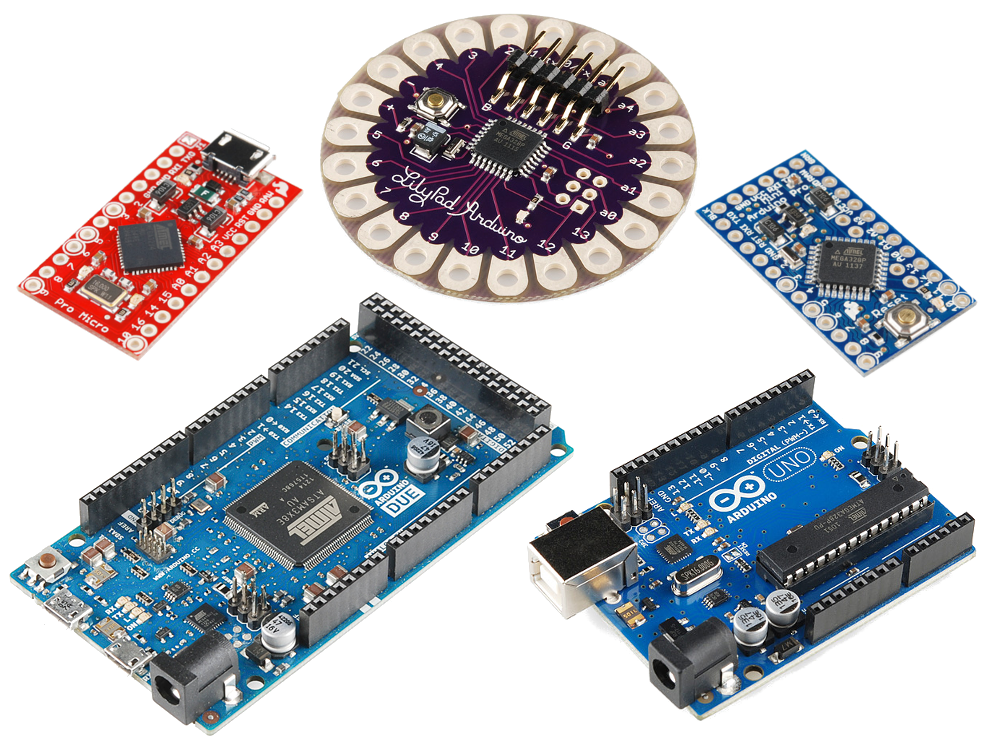
\includegraphics[height=100px]{arduinos}
\caption{ Modelos de Arduino \label{fig.arduinos} }
\end{minipage}
\begin{minipage}{0.50\textwidth}
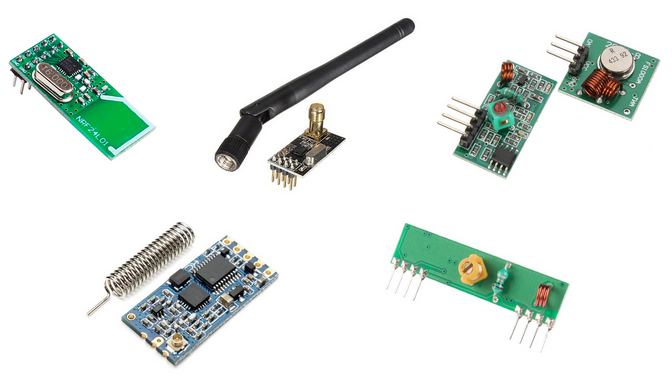
\includegraphics[height=100px]{rfs}
\caption{ Módulos RF \label{fig.rfs} }
\end{minipage}
\end{figure}

Os microcontroladores em placas compatíveis com a plataforma Arduino são os
mais populares e disponíveis no mercado brasileiro.
%
A Figura~\ref{fig.arduinos} indica alguns modelos que podem ser avaliados para
adoção no projeto (item 1).
%
Como exemplo, o modelo \emph{Pro Mini 3.3V} tem tamanho reduzido, baixo consumo
de energia e custa em torno de R\$15,00.

O levantamento, avaliação e montagem dos módulos de rádio é a etapa mais
sensível no projeto da plataforma de hardware (item 2).
%
A Figura~\ref{fig.rfs} ilustra a diversidade de implementações de módulos RF
disponíveis, alguns com custo inferior a R\$10,00.
%
Idealmente, cada um dos módulos considerados deve ser acoplável e facilmente
intercambiáveis na nossa plataforma, dado que temos como objetivo a
flexibilidade para experimentação e pesquisa em IoT.
%
Cada módulo poderá ser avaliado e desenvolvido em separado.
Para isso, iremos propor a exploração desses módulos em projetos da disciplina
de Software Embarcado em nosso programa de pós graduação.

A plataforma também deve permitir o acoplamento de sensores e outros
periféricos (item 3).
%
Além disso, deve oferecer mecanismos para desligá-los eletricamente por
software de modo a economizar energia.
%
Esses mecanismos podem usar diretamente os pinos do microcontrolador para
sensores mais simples ou transistores que funcionarão como chaves eletrônicas.
%
Esse estudo também pode ser realizado em separado por uma outra equipe.

\begin{figure}[b]
\begin{minipage}{0.50\textwidth}
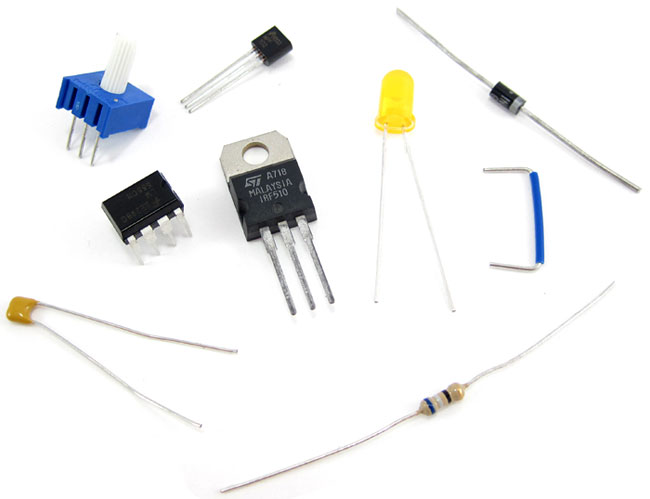
\includegraphics[height=100px]{through-hole}
\caption{ Componentes \emph{Through-Hole} }
\end{minipage}
\begin{minipage}{0.50\textwidth}
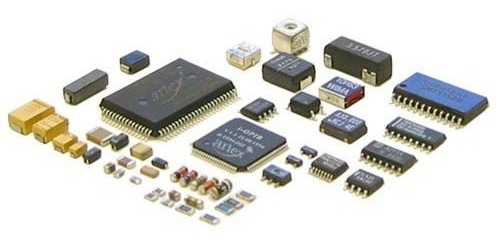
\includegraphics[height=100px]{smd}
\caption{ Componentes \emph{SMD} }
\end{minipage}
\label{fig.mount}
\end{figure}

Os componentes eletrônicos devem possuir pinos para montagem
\emph{through-hole}, como ilustrado na Figura~\ref{fig.mount}, que é a técnica
mais flexível e adequada para protótipos considerando o contexto de pesquisa.
%
Esses componentes também costumam ser mais disponíveis no mercado para compras
em pequenas quantidades.

É importante destacar que o desenvolvimento do hardware não depende da frente
de pesquisa em software em \CEU, e tampouco depende do desenvolvimento de
softwares complexos.
Como iremos utilizar hardware de commodity, já existe oferta suficiente de
bibliotecas e aplicações open-source para testes.
%
Apenas para a avaliação de consumo de energia as duas frentes deverão ser
necessariamente integradas.

Osciloscópio 3k

Serrapilheira


 do modo a permitir.



Inicialmente, não iremos considerar outras tecnologias


IMAGEM: prototipo PCB

////
////


\begin{comment}

Problemas com hardware para pesquisa científica
    - flexibilidade é importante
    - principalmente para o radio
    - custo para reproduzir
        - SoC, SMD, prontos/caros/inflexíveis
    - consumo ainda alto
        - transistores para desligar sensores
    - Solução
        - módulos off-the-shelf de fácil ligacao, jumpers/headers/solda/PCB vs SMD
        - The main advantages of SMT over the older through-hole technique are: 
            - https://en.wikipedia.org/wiki/Through-hole_technology
            - https://en.wikipedia.org/wiki/Surface-mount_technology

\end{comment}

\subsection{ Abstract (in english): }

%(Text limited to 6000 characters) characters left 

g) Etapas de execução do projeto com respectivo cronograma de atividades;
h) Produtos esperados como resultado da execução do projeto, com previsão de cronograma
de entregas anuais;
i) Potencial de impacto dos resultados do ponto de vista técnico-científico, de inovação,
difusão, sócio-econômico e ambiental;
j) Colaborações ou parcerias já estabelecidas para a execução do projeto;
k) Perspectivas de colaborações interinstitucionais para a execução do projeto;
l) Recursos financeiros de outras fontes aprovados para aplicação no projeto;
m) Disponibilidade efetiva de infraestrutura e de apoio técnico para o desenvolvimento do
projeto;
n) Orçamento detalhado.

- Até 36 meses

\bibliographystyle{plain}
\bibliography{my,other,serra} 

\end{document}
